%mark = star, diamond, square, otimes
%\documentclass{article}
%\usepackage{pgfplots}
%\usepackage[justification=centering]{caption}
%\pgfplotsset{compat=newest}
%\begin{document}
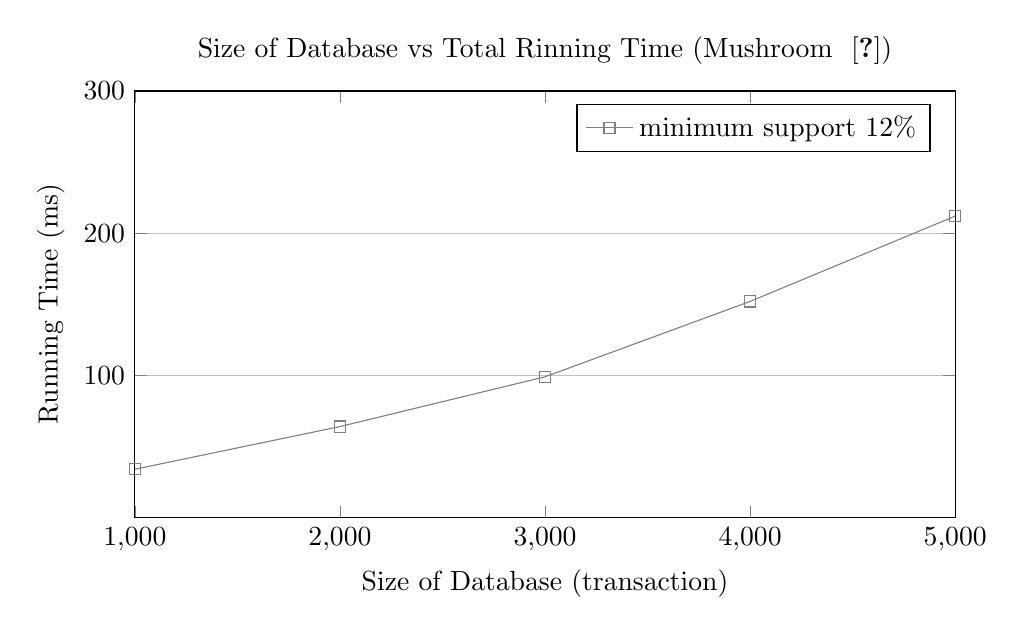
\begin{tikzpicture}
\begin{axis}[
	title={Size of Database vs Total Rinning Time (Mushroom ~\cite{dataset})},
	width=12cm,
	height=7cm,
    xlabel={Size of Database (transaction)},
    ylabel={Running Time (ms)},
    xmin=1000, xmax=5000,
    ymin=0, ymax=300,
    xtick={1000,2000,3000,4000,5000},
    ytick={100,200,300},
    legend pos=north east,
    ymajorgrids=true,
    grid style={line width=.2pt,draw=gray!50},
]
 
\addplot[
    solid,color=gray, every mark/.append style={solid, fill=gray}, mark=square
    ]
    coordinates {
		(1000,34)
		(2000,64)
		(3000,99)
		(4000,152)
		(5000,212)

	};
    \addlegendentry{minimum support 12\%}

\end{axis}
\end{tikzpicture}
%\end{document}